\documentclass{standalone}
\usepackage{tikz}
\usetikzlibrary{matrix,chains,positioning,decorations.pathreplacing,arrows}

\begin{document}

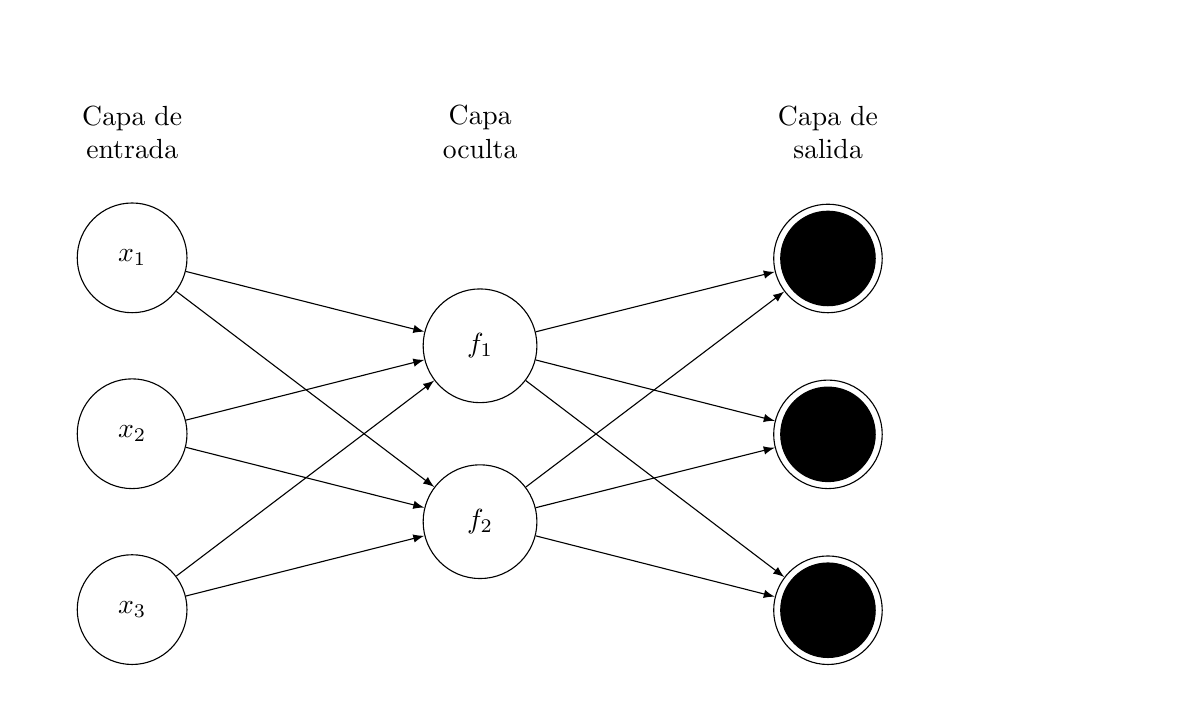
\begin{tikzpicture}[
plain/.style={
  draw=none,
  fill=none,
  },
net/.style={
  matrix of nodes,
  nodes={
    draw,
    circle,
    inner sep=10pt
    },
  nodes in empty cells,
  column sep=2cm,
  row sep=-9pt
  },
>=latex
]
\matrix[net] (mat)
{
|[plain]| \parbox{1.3cm}{\centering Capa de\\ entrada} & |[plain]| \parbox{1.3cm}{\centering Capa\\oculta} & |[plain]| \parbox{1.3cm}{\centering Capa de\\salida} \\
$x_1$ & |[plain]| & $g_1$ \\
|[plain]| & $f_1$\\
$x_2$ & |[plain]| & $g_2$ & |[plain]| \\
|[plain]| & $f_2$ \\
$x_3$ & |[plain]| & $g_3$ \\
};

\foreach \ai in {2,4,6}
{\foreach \aii in {3,5}
  \draw[->] (mat-\ai-1) -- (mat-\aii-2);
}

  
\foreach \aii in {3,5}{
  \foreach \ai in {2,4,6}{
    \draw[->] (mat-\aii-2) -- (mat-\ai-3);
  }
}

\draw [fill=black] (mat-2-3) circle [radius=0.6];
\draw [fill=black] (mat-4-3) circle [radius=0.6];
\draw [fill=black] (mat-6-3) circle [radius=0.6];

\end{tikzpicture}


\end{document}